\chapter{Case Study: Network Model Development in PTV Visum}

\section{Study Area and Data Collection \& Preparation}
The study focuses on the Southern Italy region, encompassing Molise, Campania, Puglia, Basilicata, parts of Lazio, Abruzzo, and Calabria. This area covers approximately 48,713 km² and has a total population of 9,909,625 inhabitants. The region is crucial for national transportation planning and economic connectivity, serving as a link between central Italy and key Mediterranean trade routes. However, it is also one of the most seismically active areas in the country, making the resilience of its road infrastructure a critical concern.

Seismic activity in the study area is particularly concentrated in the Campania and Calabria regions, where three major seismic fault points have been identified. These include one fault in Benevento province and another in Avellino province, both within Campania, as well as one fault in Cosenza province in Calabria. These locations are historically prone to earthquakes, which can lead to severe disruptions in road networks, bridge failures, and overall reductions in regional mobility \cite{Tang2011}. The combination of seismic hazards, complex topography, and aging infrastructure necessitates a comprehensive resilience framework for transport planning \cite{Gu2020}.

% The transportation network in Southern Italy consists of motorways, trunk roads, primary roads, and secondary roads, forming a hierarchical system that connects major urban centers with industrial and rural areas. The presence of motorway trunk roads is particularly significant as they serve as primary corridors for long-distance travel and freight transport. Ensuring the continuity and adaptability of these roads under seismic conditions is essential for maintaining regional accessibility and economic stability.

The Southern Italy road network was downloaded from OpenStreetMap (OSM) in \texttt{.osm} format and imported into PTV Visum. The 'Urban Road Network' configuration was used to ensure accurate classification of roads based on their functional hierarchy. This dataset provided detailed information on road types, connectivity, and infrastructure characteristics.
The categorization of OpenStreetMap has been used to select the roads that should be part of the final supply model since that OSM categorization refers to a specific road element in italian regulation. The match is written in the following: 

\begin{itemize}
    \item Motorway: Highway (A) including highway junctions (RA) and highway tunnels (T)
    \item Trunk: Ring road/main extra-urban road, also roads of lesser importance having interchanges rather than at-grade intersections
    \item Primary: State Road (SS) including former state roads (SS/SP/SR/SP), regional roads (SR) of great importance, provincial roads (SP) of great importance
    \item Secondary: Provincial Roads (SP) and regional roads (SR) of lesser importance
    \item Tertiary: Less important roads with a width of at least 4 meters and also main urban thoroughfares  
\end{itemize}

Additional datasets were integrated to enhance spatial accuracy and resilience assessment. KML files from Google Maps containing information on the National Autonomous Roads Corporation (ANAS) infrastructure and seismic fault locations were extracted and converted into Shapefiles using QGIS for compatibility with PTV Visum. The inclusion of ANAS-managed roads was necessary as these routes form key transport corridors maintained by Italy’s national highway agency, ensuring connectivity across the region. The seismic fault dataset provided a detailed representation of earthquake-prone zones, enabling an in-depth analysis of network vulnerabilities in relation to these fault lines \cite{Zeng2021}.

Once processed, the Shapefiles were integrated into PTV Visum to allow for comprehensive network analysis and simulation. The study considers the impact of earthquake-induced road disruptions, focusing on identifying critical links that may require infrastructure reinforcement, redundancy planning, or alternative routing strategies. The structured combination of road network data, seismic risk information, and transport infrastructure attributes enables an evaluation of network resilience and redundancy, offering insights for transport planning and disaster preparedness in Southern Italy.

\section{Zoning for Transportation Analysis}
With regards to zoning, the starting point was the census district data for Lazio, Abruzzo, Molise, Campania, Puglia, Basilicata, and Calabria at the smallest geographical level (named \textit{sezioni censuarie in Italian} that were sourced from the Italian National Institute of Statistics (ISTAT). Based on \textit{sezioni censurie} an aggregation activity has been made based on the belonging to the same village. The key attributes used for this operation was the municipal code (Procom for ISTAT). According to this criteria, in the study area has been identified 1,242 Territories that were too many first for transportation reason and also due to license constraints (the limit is of 1000 traffic zones. For this reasons adjustments were necessary.
Starting from municipality zoning, some of them has been aggregated while some other once has been splitted according to density, population and area. In detailed, the criteria are reported in the following.\\

To identify the villages that should be aggregate he following criteria were used:
\begin{itemize}
    \item \textbf{Population Density:} Territories with less than 30 inhabitants per km² were merged.
    \item \textbf{Population Size and Area:} Territories with a population below 2,000 and an area greater than 5 km² were merged.
\end{itemize}
Once zones has been identified, natural features (e.g., rivers) and infrastructural elements (e.g., railway lines) were used as boundaries for aggregation to define new traffic zones. This approach aligns with recommended practices to ensure that centroid connectors do not unrealistically cross physical barriers, thereby maintaining logical accessibility within the model \cite{Cambridge2007}. Zones divided by barriers were ensured to have adequate crossing points (e.g., bridges, underpasses) to maintain connectivity. This process joined 570 villages into 68 zones.\\
To identify the villages that should be splitter the following criteria were used:
\begin{itemize}
    \item \textbf{High-Density Areas:} Zones with more than 1,000 inhabitants per km² and an area exceeding 10 km² were divided.
    \item \textbf{Significant Urban Centers:} Major urban areas, such as provincial capitals, were split to reflect complex travel dynamics.
\end{itemize}

Internal barriers such as rivers or railways were considered, and zones were split along these features unless sufficient infrastructure (e.g., multiple bridges or crossings) ensured connectivity. 
Based on this criteria Fifty-four villages were split creating 150 traffic zones\\
City centers were identified within each zone to ensure accessibility and accurate representation of travel origins and destinations. Each zone required at least one link connecting it to the major road network. Zones isolated by rivers or railways without adequate crossings were adjusted to reflect realistic travel paths. At the end, has been defined 778 traffic zones in the study area.\\
Lastly, the network was filtered to retain only essential road types, including motorways, trunk roads, and primary, secondary, and tertiary roads. Some unclassified one-lane and residential roads were retained if essential for connectivity. Unnecessary links within zones were removed, ensuring that each zone had at least one connection to the major road network.
The supply model and zoning are reported in \ref{fig:supplymodel} e \ref{fig:zoning}

\begin{figure}
\centering
{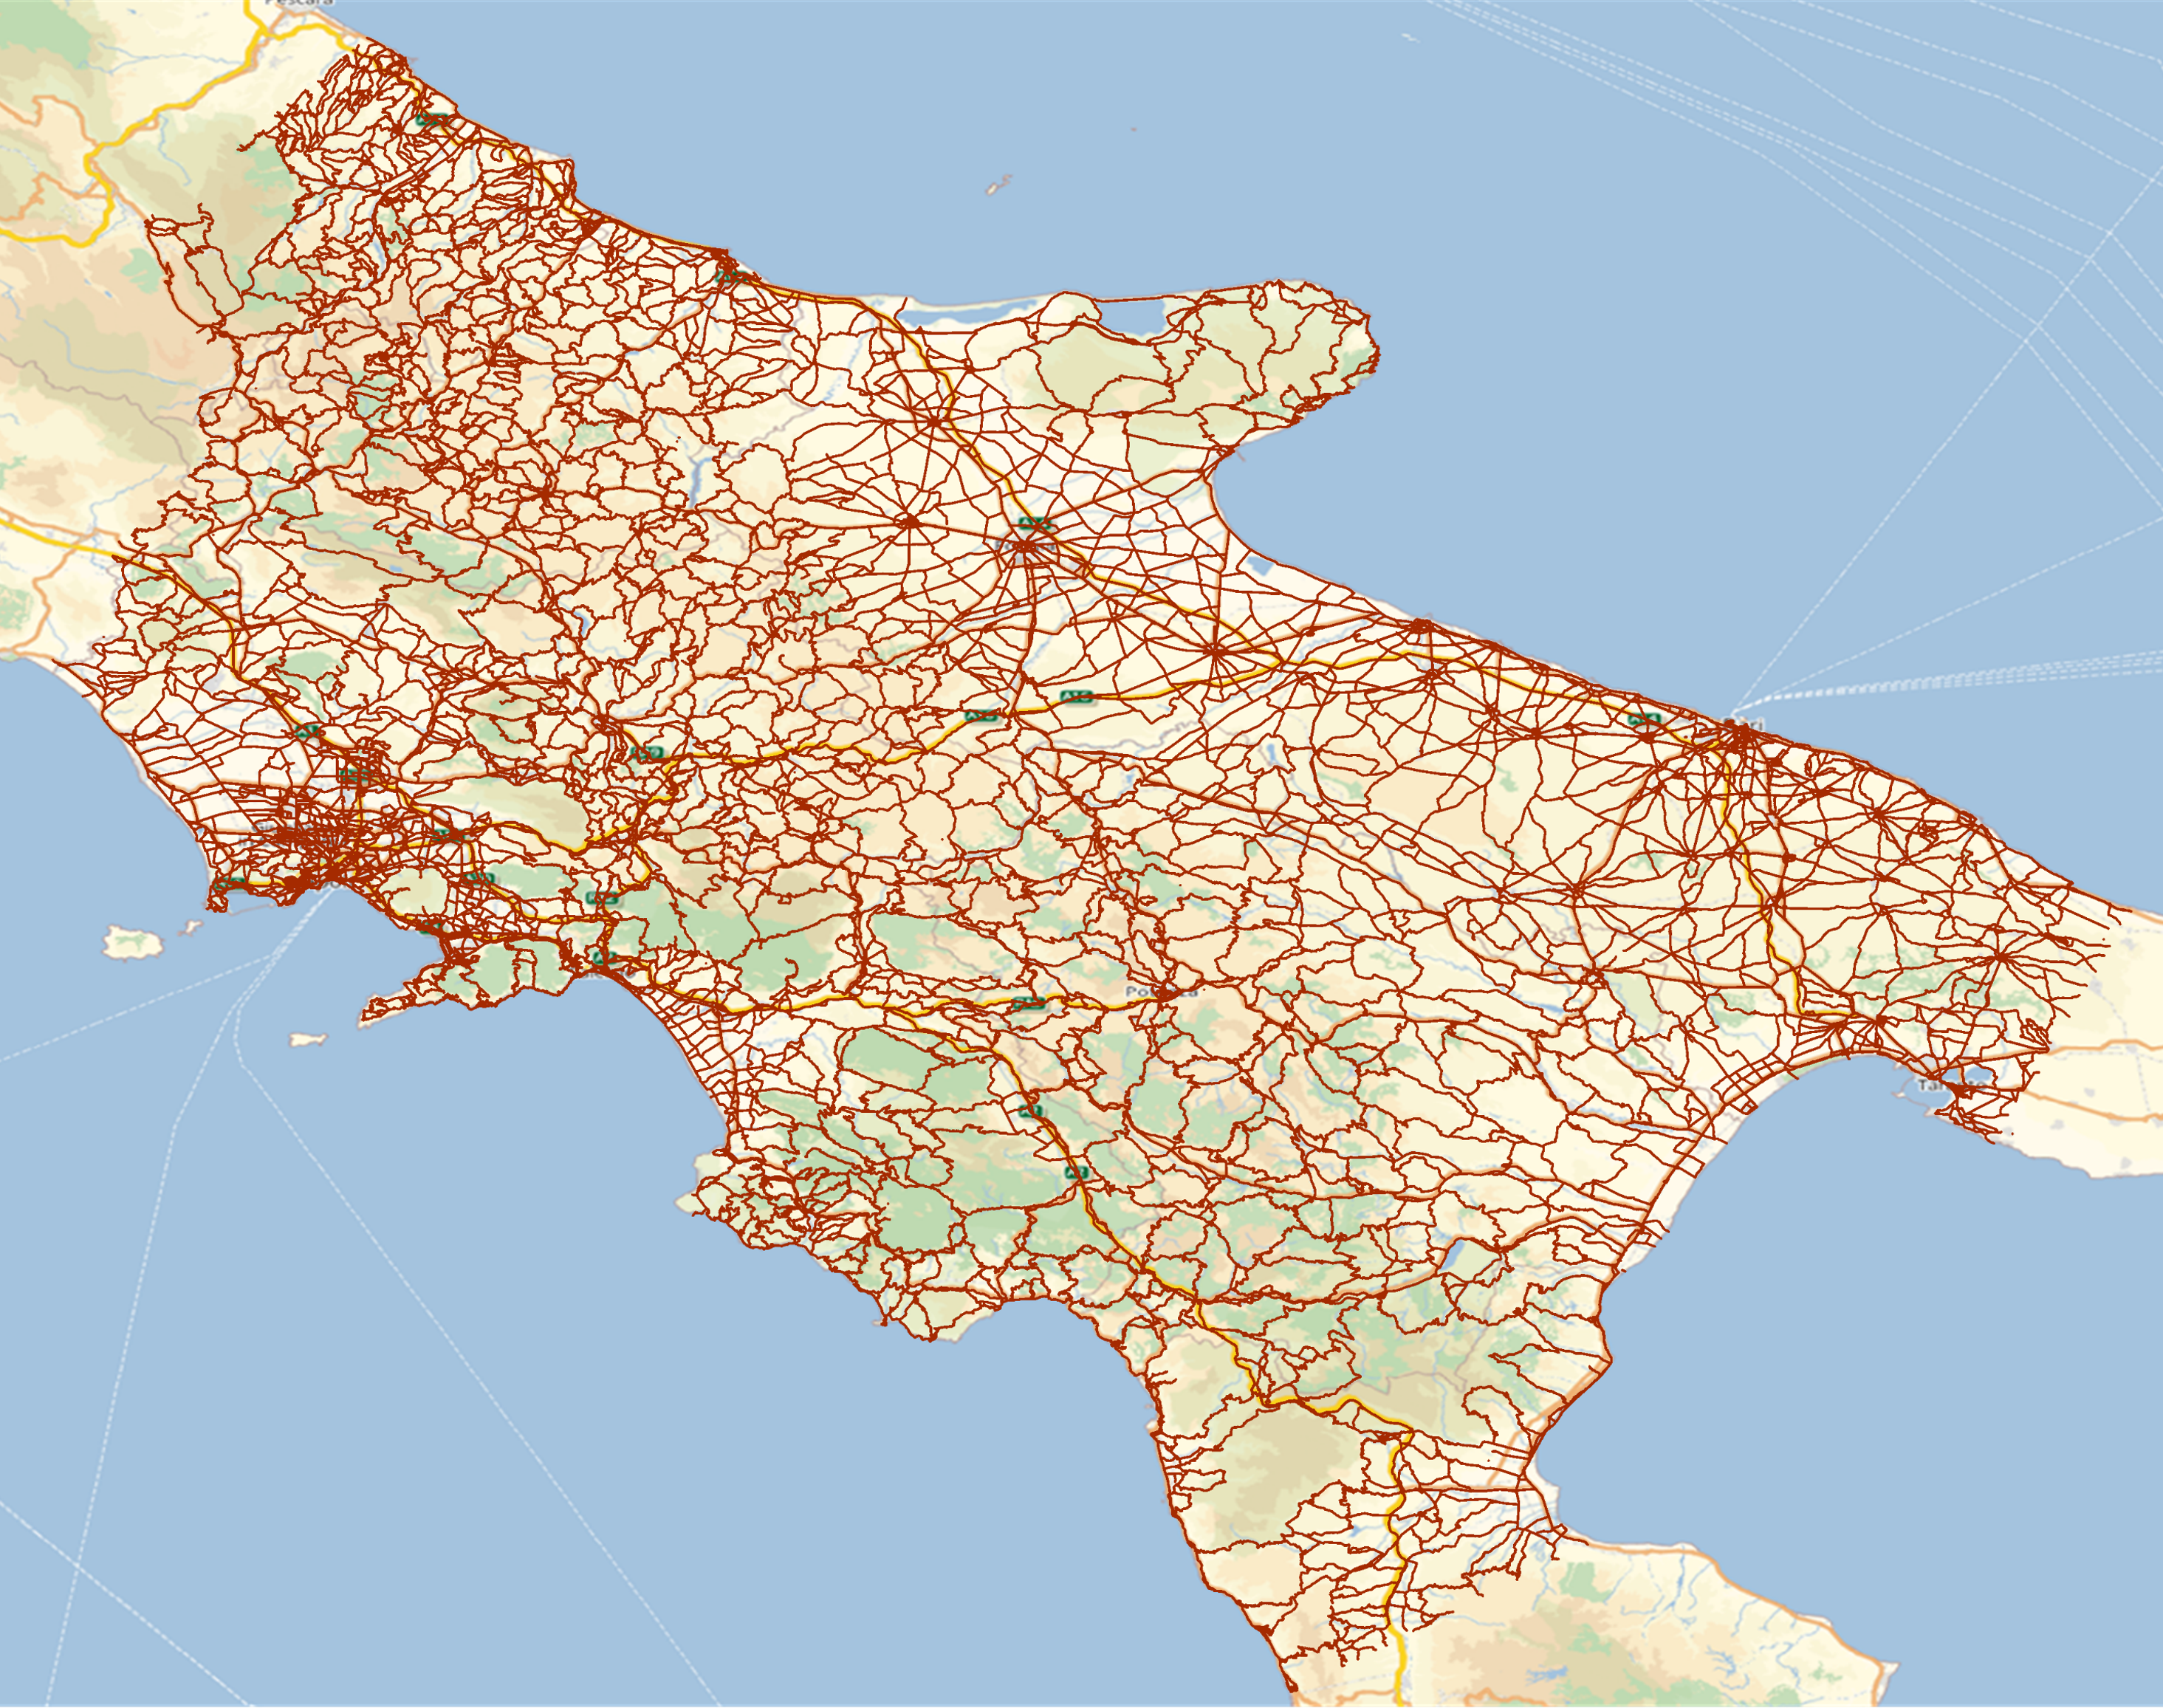
\includegraphics[width=.90\textwidth]{images/SupplyModel.png}}
    \caption{Supply Model for study area}
    \label{fig:supplymodel}
\end{figure}

\begin{figure}
\centering
{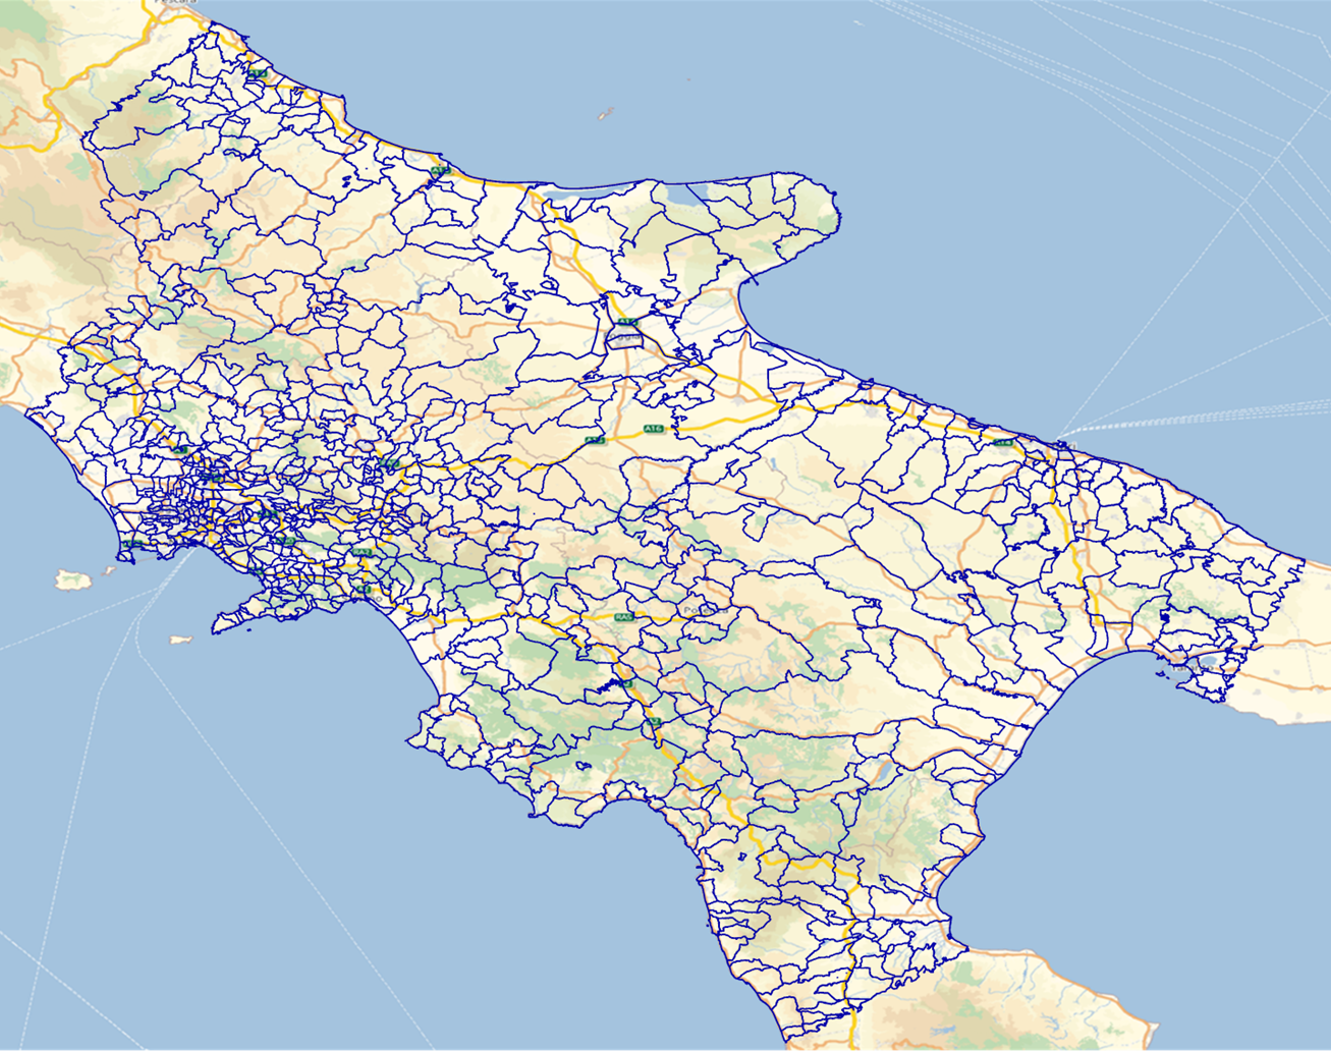
\includegraphics[width=.90\textwidth]{images/Zoning.png}}
    \caption{Zoning for study area}
    \label{fig:zoning}
\end{figure}

\section{Supply Model Development – Adjusting Free Flow Speeds in PTV Visum}
Accurate free-flow speed calibration is a critical aspect of transport modeling, ensuring that simulated traffic conditions reflect real-world driving behavior.Given the geographical and infrastructural characteristics of the Southern Italy study area, particularly in mountainous terrains and city centers, modifying the default speed limits in PTV Visum was necessary. Many tertiary and secondary roads had unrealistic speed limits (80–100 km/h), leading to inaccurate travel time estimations and unreliable network performance assessments. A systematic approach was implemented to filter, analyze, and reclassify road speeds based on road characteristics, naming conventions, and functional classifications.

\subsection{Identifying Misclassified Roads and Need for Speed Adjustments}
Upon importing the OpenStreetMap (OSM) road network into PTV Visum, initial observations revealed that many roads were assigned unrealistic speed limits. Mountainous roads, urban roads, and roads with high curvature often had speeds set at 80–100 km/h, which is not practical. Urban streets labeled “Via” or “Viale” had excessive speed limits, despite their functional characteristics suggesting lower speeds due to congestion, pedestrian activity, and intersections. Provincial and national roads (Provinciale, Statale) required further verification, as their design speeds varied significantly based on location and function. Since speed is a crucial factor in calculating shortest paths, travel times, and overall network efficiency, realistic speed calibration was necessary.

\subsection{Filtering and Reclassification Process in PTV Visum}
A structured approach was followed to identify and correct misclassified roads. First, tertiary and secondary roads with speeds between 80–100 km/h were extracted and manually reviewed. Each road segment was evaluated based on geometry, surrounding environment, and road naming conventions.\\
Curved, winding roads and irregular alignments were considered unsafe for high-speed driving and downgraded to 60 km/h where necessary. Urban roads, particularly those inside city centers, were reassigned 60 km/h speed limits, while highway-style rural roads with minimal intersections and wider lanes were preserved at higher limits. Roads labeled “Via” or “Viale” typically serve mixed-use areas with high pedestrian and vehicular interaction and were reclassified to 60 km/h. Provincial and national roads (Strade Provinciali - SP, Strade Statali - SS) were also reclassified: SP roads in urban/peri-urban areas were reduced to 60 km/h, while rural SP roads were kept at 90 km/h. SS roads were maintained at 90 km/h, depending on function and road width.\\
A final manual verification step was conducted, ensuring the new speed values matched real-world conditions. Road classifications were visually inspected in PTV Visum and compared with official Italian speed limits.

\subsection{Consideration of Road Characteristics and Functional Classes}
Beyond speed limits, additional factors were considered to improve model accuracy. Mountainous and hilly terrains were assigned lower speed classifications due to sharp turns and elevation changes. Roads with steep gradients and hairpin turns were reclassified to 60 km/h. High-traffic urban roads, even if categorized as secondary or tertiary roads, were also set at 60 km/h due to congestion.

\section{Validation of Speed Assumptions (Supply Model Validation)}
\subsection{Selection of Origin-Destination (OD) Pairs}
A total of 84 OD pairs were chosen across 58 zones to encompass diverse regions and travel conditions reported in \ref{fig:zones modelvalidation}. This included 18 OD pairs from provincial capitals to ensure a mix of urban and interregional routes. Additional OD pairs were strategically placed to cover different road types, variations in free-flow speed, and locations between seismic faults to assess network resilience.
The comparison has been made on uncongested travel time using data obtained by Google Maps (that represent our real data) and the ones obtained by the model. The data collected by Google used a query where the starting time was settled at 1–2 AM to ensure minimal congestion effects, aligning with the model's free-flow conditions

\begin{figure}
\centering
{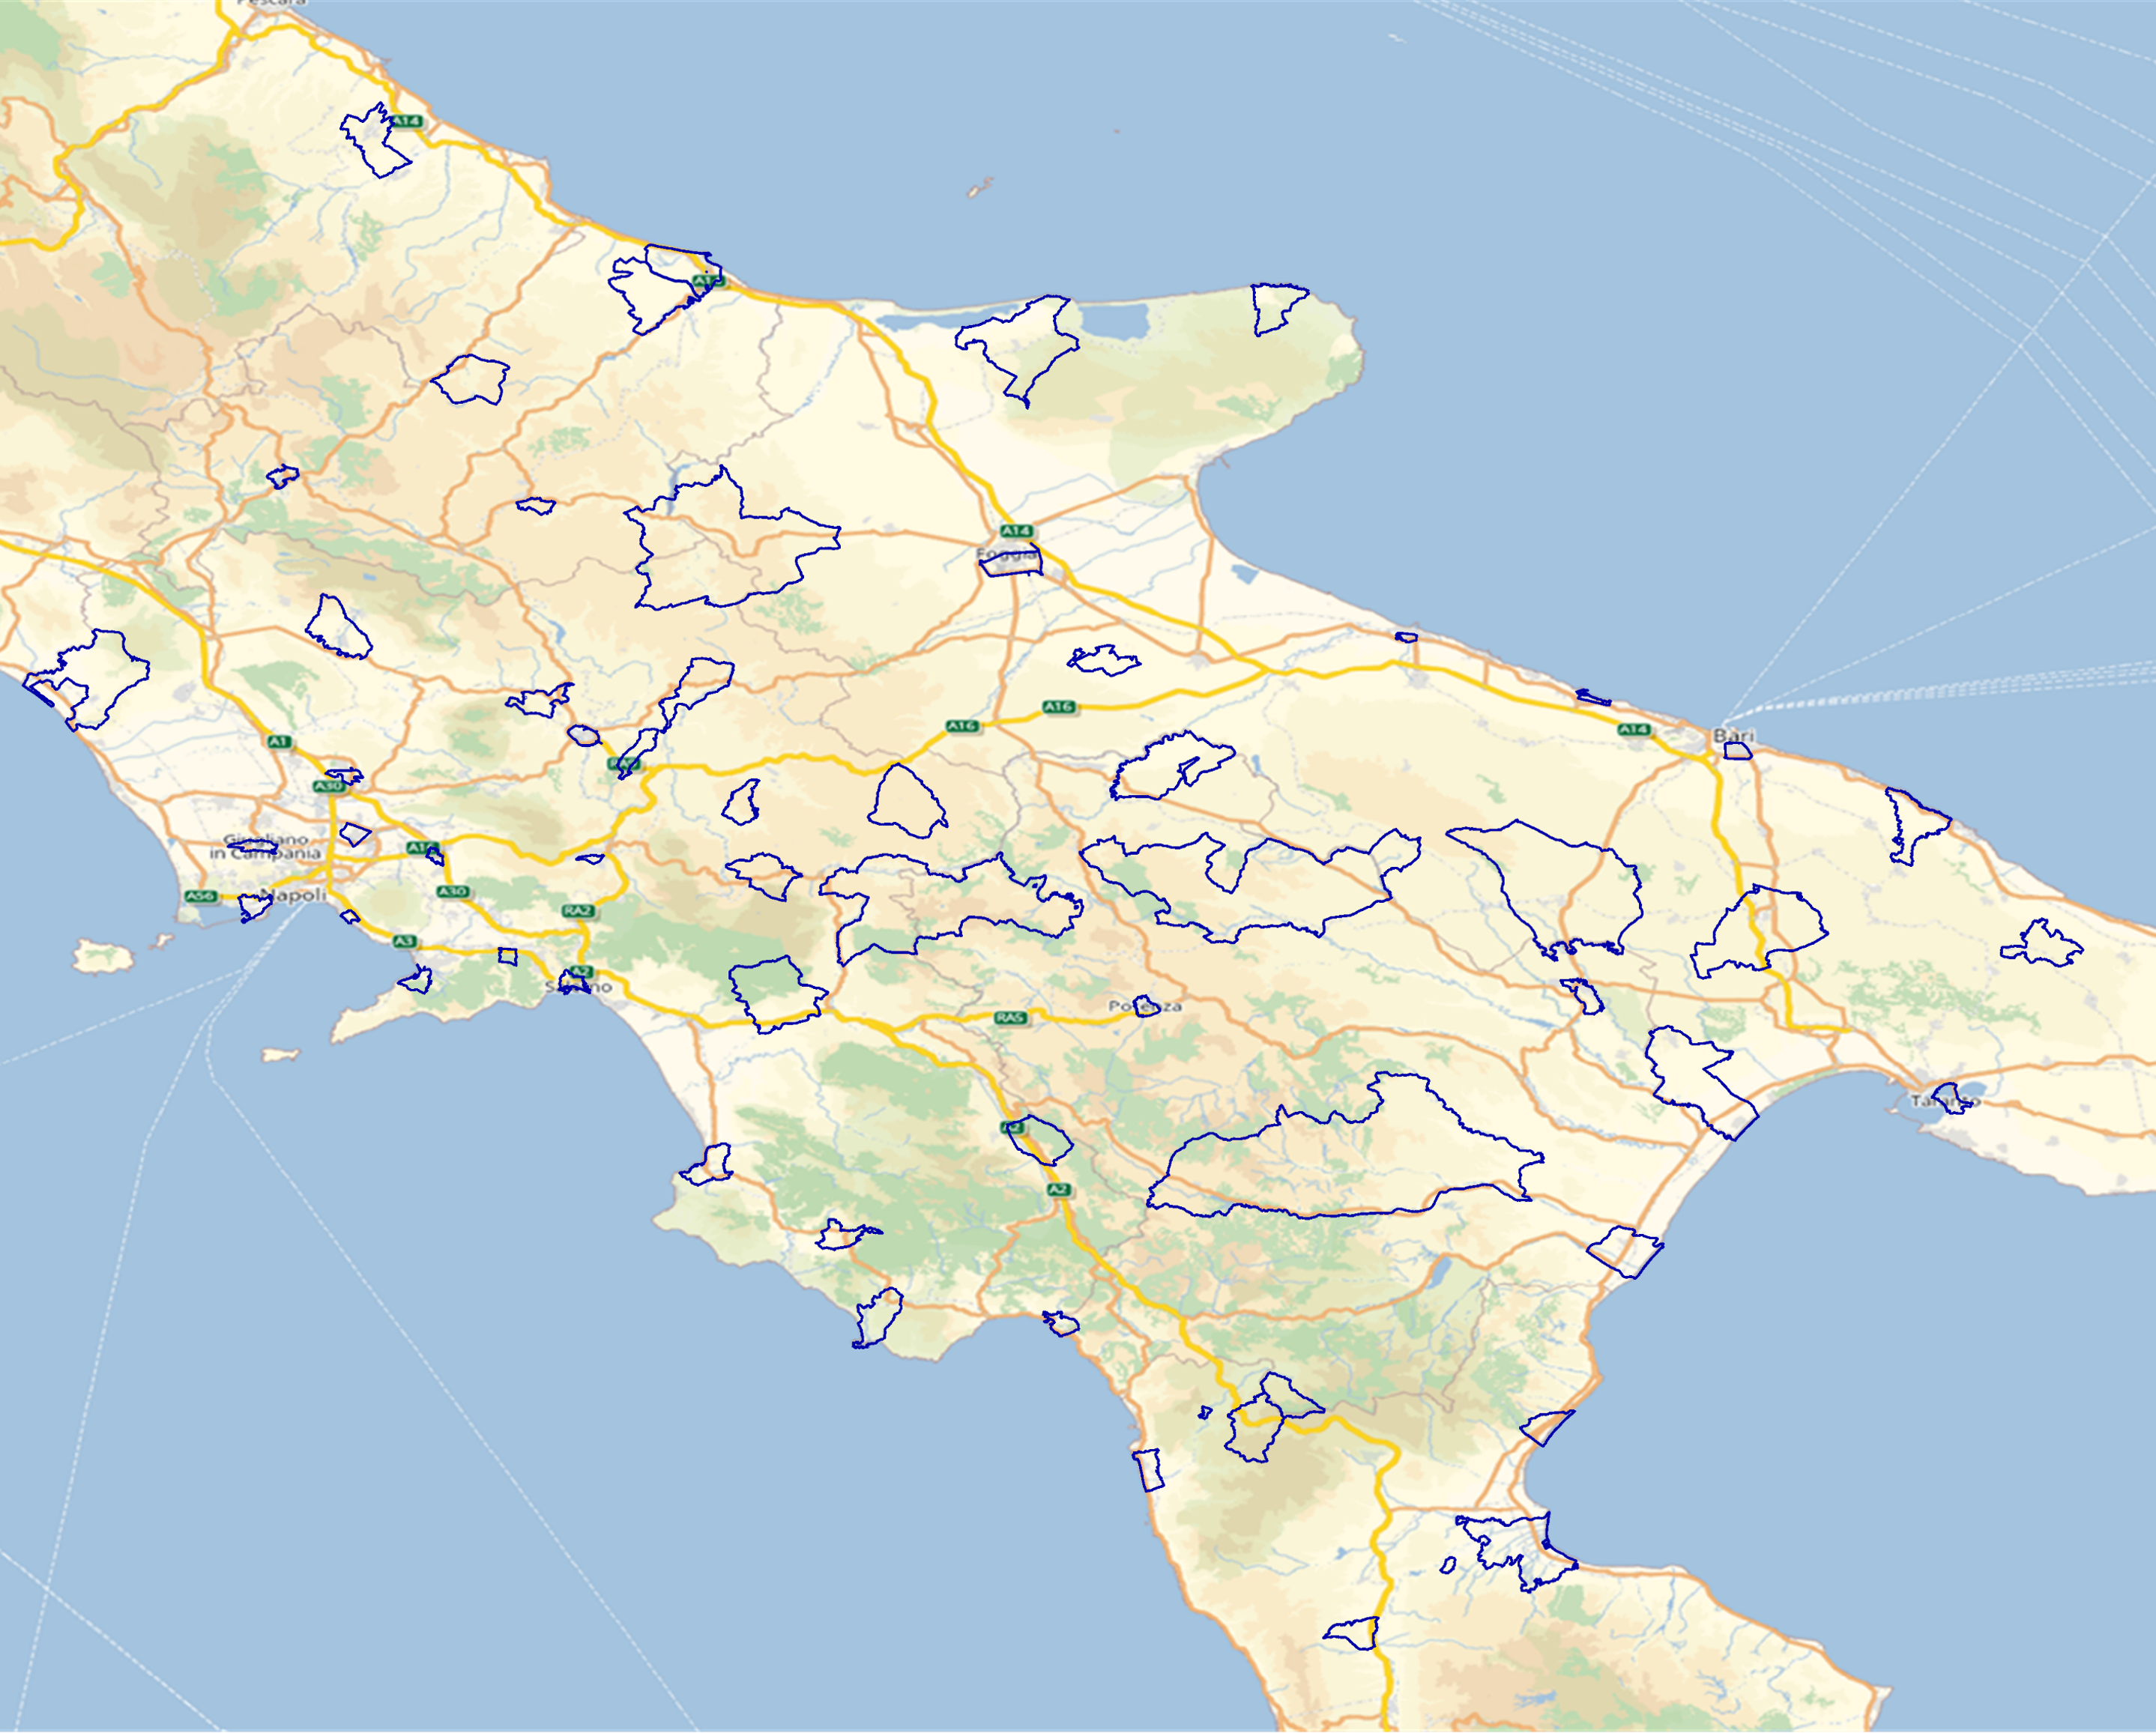
\includegraphics[width=.8\textwidth]{images/Validation_zones.png}}
    \caption{Zones used for validating the model}
    \label{fig:zones modelvalidation}
\end{figure}

\subsection{Data Analysis and Validation Results}
A scatter plot was generated to compare travel times from PTV Visum with those from Google Maps. Linear regression analysis yielded the equation:
\begin{equation}
y = 0.9684x + 5.9104
\end{equation}

where \( y \) represents PTV Visum travel time and \( x \) represents Google Maps travel time. The coefficient (0.9684) indicated that PTV Visum travel times were closely aligned with real-world data, and an \( R^2 \) value of 0.9779 confirmed strong correlation.Most OD pairs had errors within $\pm 10$--$15\%$, which was within an acceptable validation range. A few outliers with deviations above $20\%$ indicated potential local variations in speed assumptions.
A graphical representation of regression are shown in 

\begin{figure}
\centering
{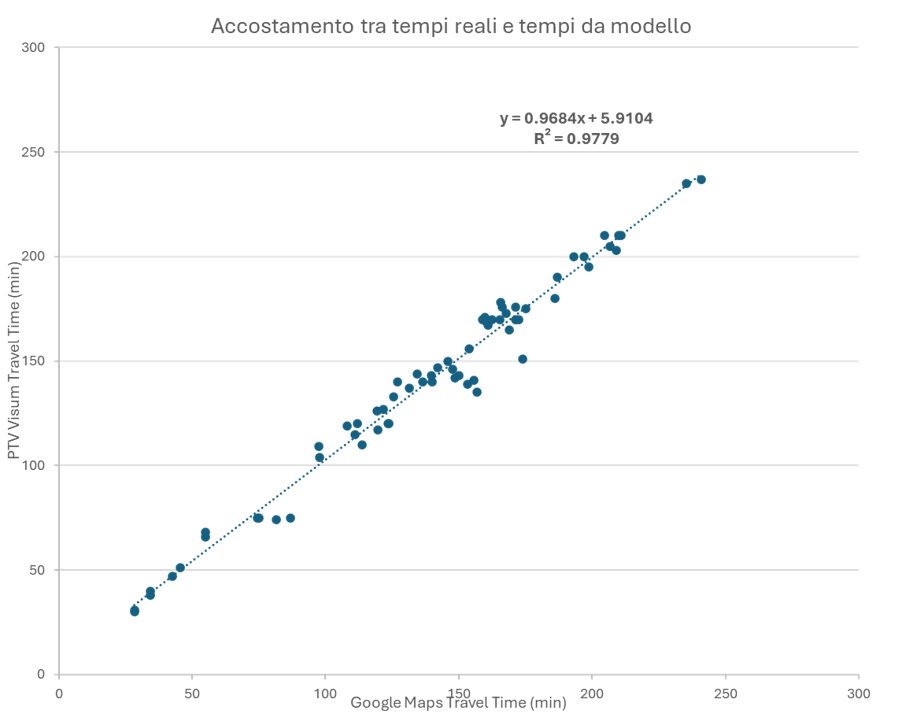
\includegraphics[width=.8\textwidth]{images/Validation_results.png}}
    \caption{$R^2$ between uncongested travel time}
    \label{fig:modelvalidation}
\end{figure}

\subsection{Implications of Speed Adjustments for the Supply Model}
By refining free-flow speeds, the transport model in PTV Visum now provides:
\begin{itemize}
    \item More realistic travel times, improving the accuracy of traffic assignment models.
    \item Better route selection behavior, reducing overestimation of highway usage in mountainous and urban areas.
    \item Stronger validation with real-world data, ensuring network performance indicators (e.g., betweenness centrality, connectivity, and redundancy) are correctly represented.
\end{itemize}

\section{Seismic Disruption Scenarios and Network Impact Analysis}

Assessing the impact of seismic events on transportation networks is crucial for understanding network resilience and planning effective mitigation strategies. In this context, redundancy indicators such as the beta index, gamma index, betweenness centrality, average degree, and clustering coefficient are essential metrics that provide insights into network connectivity, complexity, and robustness. This section outlines the methodology used to model seismic disruptions, evaluate their effects on the transport network, and analyze key resilience indicators.

\subsection{Seismic Fault Impact Scenarios}

To assess the impact of seismic events on the transport network, two disruption scenarios were defined for each of the three identified seismic fault points in Southern Italy. These scenarios were designed to represent varying levels of earthquake intensity and their corresponding effects on road infrastructure.

The disruption scenarios were defined as follows:
\begin{itemize}
    \item \textbf{Low-intensity earthquake}: 10 percent of road links within an 8 km radius of the fault point were disrupted.
    \item \textbf{High-intensity earthquake}: 40 percent of road links within a 15 km radius of the fault point were disrupted.
\end{itemize}

To identify affected road links, QGIS spatial analysis was used to create buffer zones of 8 km and 15 km radii around each seismic fault point. All road links within these buffer zones were extracted, and a random selection process was applied to disrupt 10 percent of links in the low-intensity scenario and 40 percent in the high-intensity scenario. This random selection simulates the unpredictable nature of earthquake-induced infrastructure failures.

These selected disrupted links were then imported into PTV Visum for network disruption modeling. In PTV Visum, disruptions were applied by setting the capacity (CapPrT) of the affected links to 0, simulating their failure and removal from the network. This process allowed for the assessment of network performance under earthquake conditions, identifying changes in connectivity, alternative routing possibilities, and potential congestion zones.


